%%%%%%%%%%%%%%%%%%%%%%% file main.tex %%%%%%%%%%%%%%%%%%%%%%%%%
% Tolga Acar's contribution to Special edition in JCEN to honor Peter L. Montgomery
% September 2016
%%%%%%%%%%%%%%%%%%%%%%%%%%%%%%%%%%%%%%%%%%%%%%%%%%%%%%%%%%%%%%%%%%%
%
\RequirePackage{fix-cm}
%
%\documentclass{svjour3}                     % onecolumn (standard format)
%\documentclass[smallcondensed]{svjour3}     % onecolumn (ditto)
%\documentclass[smallextended]{svjour3}       % onecolumn (second format)
\documentclass[twocolumn]{svjour3}          % twocolumn
%
\smartqed  % flush right qed marks, e.g. at end of proof
%
\usepackage{graphicx}
\usepackage[linesnumbered,ruled]{algorithm2e}
\usepackage{listings,multicol,multirow}
%
% \usepackage{mathptmx}      % use Times fonts if available on your TeX system
%
% insert here the call for the packages your document requires
%\usepackage{latexsym}
% etc.
%
% please place your own definitions here and don't use \def but
% \newcommand{}{}
%
% Insert the name of "your journal" with
\journalname{JCEN}
%
\begin{document}

\title{Montgomery Multiplier in Software%\thanks{Grants or other notes
%about the article that should go on the front page should be
%placed here. General acknowledgments should be placed at the end of the article.}
}
%\subtitle{Do you have a subtitle?\\ If so, write it here}

%\titlerunning{Short form of title}        % if too long for running head


\author{Tolga Acar \and Erdinc Ozturk}

%\authorrunning{Short form of author list} % if too long for running head

\institute{
T. Acar \at
              Microsoft \\
              \email{tolga@microsoft.com}            \\
              \emph{One Microsoft Way, Redmond, WA 98052}
\and 
Erdinc Ozturk \at
              Istanbul Commerce University \\
              \email{erdinco@gmail.com}
}

\date{Received: date / Accepted: date }
% The correct dates will be entered by the editor


\maketitle

\def\bfor{\bf for\hspace{1ex}}
\def\bto{\hspace{1ex}\bf to\hspace{1ex}}
\def\bif{\bf if\hspace{1ex}}
\def\bthen{\hspace{1ex}\bf then\hspace{1ex}}
\def\belse{\bf else\hspace{1ex}}
\def\bret{\bf ret\hspace{1ex}}

\newcommand{\mon}{\mbox{MonPro}}
\newcommand{\mwbox}[1]{\mbox{\hspace*{1ex}\mbox{#1}\hspace*{1em}}}
\newcommand{\eqref}[1]{\mbox{(\ref{#1})}}

\begin{abstract}

Most computer and network security systems utilizes cryptographic functions
to provide numerous security value propositions.
Software implementations of these functions
are often desired because of their flexibility and cost effectiveness.
We concentrate on developing high-speed and memory-efficient modular
multiplication and exponentiation algorithms for number-theoretic
cryptosystems.

Several cornerstone algorithms, such as RSA and Diffie-Hellman, require
modular exponentiation, which is typically broken into a series of
modular multiplications.  One of the most interesting advances in
modular exponentiation has been the introduction of Montgomery
multiplication. Our focus is squrely on the software engineer designing,
implementing, testing, shipping, maintaining, improving, and iterating on such algorithms.
We are interested in two aspects: development of fast and convenient software
methods, and balanced utilization of hardware features to achieve
high-performance algorithms.

\keywords{Montgomery \and multiplication \and exponentiation \and arithmetic }
% \PACS{PACS code1 \and PACS code2 \and more}
% \subclass{MSC code1 \and MSC code2 \and more}
\end{abstract}

% The first (Introduction) chapter of the thesis
% This is the Introduction chapter

\section{Introduction}
\label{introduction}

Public key algorithms are the foundational pieces of Internet security
protocols. Performance has always been an issue, requiring engineers
invent and develop new methods for high-speed implementations.  The
computational cost of software cryptography is a function of the
underlying algorithm and the quality of the implementation of the
algorithm \cite{RC93:A}. For the most pervasive algorithms such as RSA
algorithm \cite{RSA78:A}, the Diffie-Hellman key exchange scheme
\cite{DH76:New}, large integer multiplication and exponentiation are
the most CPU intensive operations.

When we investigate fast modular multiplication algorithms, the
Montgomery multiplication algorithms has been the cornerstone of
numerous implementations both academically and commercially.
Certainly, one of the most interesting advances in modular
exponentiation has been the introduction of Montgomery multiplication
\cite{M85:Modular}.  It became {\em de facto} algorithm in any
cryptographic method utilizing modular multiplication, especially the
RSA cryptosystem \cite{AKP96:Public,BK95:Fast}.  We are interested in
two aspects of modular multiplication algorithms: development of fast
and convenient methods on a given hardware platform, and hardware
requirements to achieve high-performance algorithms.
We provide simple ALU-based implementations as well as
vectorized and parallel implementations of the algorithm \cite{GK12:Software,PS04:Parallel}.

We discuss several Montgomery multiplication algorithms
\cite{M85:Modular}.  We discuss and analyze five time and memory
efficient algorithms.

We caution the implementer to take precautions to prevent or minimize
side channel leakage. The final conditional subtraction has been the focus
of leakage studies, and has been analyzed by Walter \cite{W08:Leakage}.

\section{Algorithms for Montgomery Multiplication}

We describe and analyze several algortihms~\cite{KAK96:Analyzing}. 
%The analyses and actual performance results indicate that the Coarsely Integrated Operand Scanning (CIOS) method is the most efficient of all five algorithms, at least for the general class of processorconsidered.
Various hardware algorithms for modular multiplication have been
proposed and some of them have been realized
\cite{B89:A,T91:A,OK91:A}.  Modular exponentiation algorithms using
division chains \cite{W97:Exponentiation}, a double-base number system
\cite{DJM97:Theory}, and complex arithmetic \cite{DJM97:Algorithms}
are applicable to software implementations. However, these methods
concentrate on fast modular exponentiation, not on the particular
modular multiplication method employed.

The Montgomery multiplication algorithm is used to speed up the
modular multiplications as well as squarings required during the
exponentiation process. The Montgomery algorithm computes
%
\begin{equation}
\mon(a,b)=a \cdot b \cdot r^{-1} \bmod{n}
\label{monpro1}
\end{equation}
%
given $a,b<n$ and $r$ such that $\gcd(n,r)=1$. Even though the
algorithm works for any $r$ which is relatively prime to $n$, it is
more useful when $r$ is taken to be a power of 2. In this case, the
Montgomery algorithm performs divisions by a power of 2, which is an
intrinsically fast operation on general-purpose computers, e.g.,
signal processors and microprocessors; this leads to a simpler
implementation than ordinary modular multiplication, which is
typically faster as well \cite{NMR95:Can}.

\subsection{Multi-Precision Multiplication}
Multiplication of two numbers smaller than the machine word-size is trivial for any machine with a core multiplier. Usually, the machine's core multiplier can multiply two word-sized numbers with a 1 cycle/multiply throughput. However, multiplication of numbers larger than the machine word size becomes a challenge for any programmer as the size of the operands grow. Multi-precision arithmetic involves operations on numbers larger than the machine word size. Since multiplication is a very time-consuming and challenging arithmetic operation, we deal with multi-precision multiplication operation in this section. In the remainder of the paper, we define a large number as any value that doesn't fit in a machine word.

There are multiple methods of efficiently multiplying two large numbers. Karatsuba-Ofman Algoritm \cite{karatsuba} and FFT-Based Multiplication Algorithm \cite{Schonhage1971} are examples that can be listed among the classical school-book multiplication algorithms. Even though these complicated algorithms have potential for more efficient implementations, we focus on the classical school-book multiplication algorithm. 

We assume that the multiplicant and multiplier have the same length, which is a more realistic case for public-key applications. However, the methods discussed here can be easily adapted for different-sized numbers. For simplicity, we pick the 64-bit word size common in modern processors without loss of generality. Assume we multiply two $n$-word numbers $A$ and $B$ where $A = (A_{n-1}A_{n-2}...A_1A_0)_b$ and $B = (B_{n-1}B_{n-2}...B_1B_0)_b$ and $b=2^{64}$. Multiplication of two unsigned integers are given in Algorithm \ref{alg:mult}. 

\begin{algorithm}
\label{alg:mult}
\caption{Classical school-book multiplication algorithm}
\SetKwInOut{Input}{Input}
\SetKwInOut{Output}{Output}
\underline{MontMul} $(A,B,N)$\;
\Input{$k$-bit integers $A=(A_{n-1}...A_1A_0)_b$, $B=(B_{n-1}...B_1B_0)_b$, $b=2^{64}$}
\Output{$C = AB$}
$\textit{t} \gets 0$ ($t=(t_{2n-1}...t_1t_0)_b$)\\
\For{i from 0 to n-1}{
	$\textit{$(t_{i+n}t_{i+n-1}...t_{i+1}t_i)_b$} \gets \textit{$(0t_{i+n-1}...t_{i+1}t_i)_b+A_iBb^i$}$ \\

}
\end{algorithm}

Algorithm \ref{alg:mult} is illustrated in Figure \ref{fig:mult} for the multiplication of two 512-bit numbers.
%
We use the term \textit{diagonal} when referring to $A_iB$ since the multiplication looks like a diagonal in Figure \ref{fig:diag0} later in the paper.

\begin{figure}
\centering
  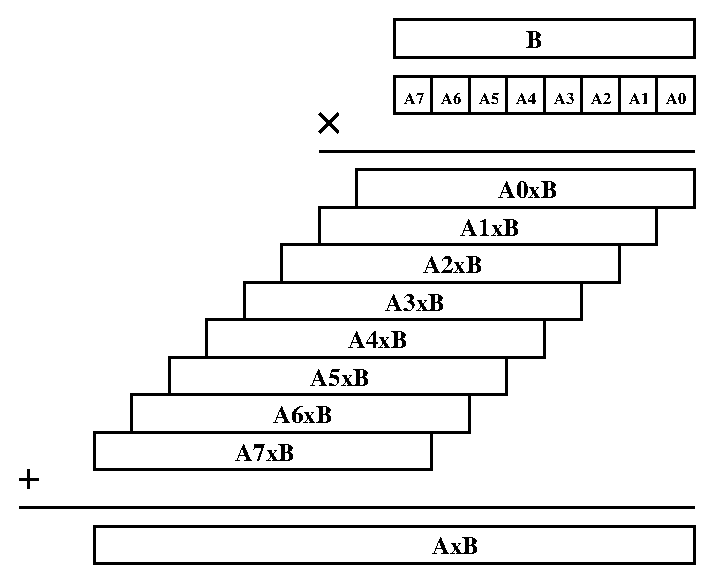
\includegraphics[scale=0.7]{mul.eps}
\caption{Classical Multiplication of two 512-bit numbers.  }
\label{fig:mult}
\end{figure}

\subsection{Montgomery Multiplication}

Let the modulus $n$ be a $k$-bit integer, i.e., $2^{k-1} \leq n < 2^k$,
and let $r$ be $2^k$. The Montgomery multiplication algorithm requires
that $r$ and $n$ be relatively prime, i.e., $\gcd(r,n)=\gcd(2^k,n)=1$,
which is easily satisfied for odd $n$.
A modified Montgomery multiplication has also been introduced for an
even modulus~\cite{K94:Montgomery}.
In order to describe the Mongtomery multiplication algorithm, we first
define the $n$-residue of an integer $a<n$ as
$\bar{a}=a \cdot r \pmod{n}$.
It is straightforward to show that the set
\[
\{~ a \cdot r \bmod{n} ~|~ 0 \leq a \leq n-1 ~\}
\]
is a complete residue system, i.e.,
it contains all numbers between $0$ and $n-1$.
Thus, there is one-to-one correspondence between the numbers in the range
$0$ and $n-1$ and the numbers in the above set. The Montgomery reduction
algorithm exploits this property by introducing a much faster
multiplication routine which computes the $n$-residue of the product of
the two integers whose $n$-residues are given.
Given two $n$-residues $\bar{a}$ and $\bar{b}$,
the Montgomery product is defined as the $n$-residue
%
\begin{equation}
\bar{c}=\bar{a} \cdot \bar{b} \cdot r^{-1} \pmod{n} \label{monp}
\mwbox{,}
\end{equation}
%
where $r^{-1}$ is the inverse of $r$ modulo $n$, i.e., it is the number with
the property $r^{-1} \cdot r = 1 \pmod{n}$.
The resulting number $c$ in \eqref{monp} is
the $n$-residue of the product $c=a \cdot b \pmod{n}$, since
%
\begin{eqnarray*}
\bar{c} & = & \bar{a} \cdot \bar{b} \cdot r^{-1} \pmod{n} \\
        & = & a \cdot r \cdot b \cdot r \cdot r^{-1} \pmod{n} \\
        & = & c \cdot r \pmod{n} \mwbox{.}
\end{eqnarray*}
%
In order to describe the Montgomery reduction algorithm, we need an additional
quantity, $n'$, which is the integer with the property
$r \cdot r^{-1} - n \cdot n' = 1$.
The integers $r^{-1}$ and $n'$ can both be computed by the extended
Euclidean algorithm \cite{K81:Seminumerical,R93:Elementary}.
The computation of $\mon(\bar{a},\bar{b})$ is achieved as follows:

\begin{tabbing}
\hspace*{.2in}\={\bf function}\= ~MonPro($\bar{a},\bar{b}$)\\
\>Step 1. $t := \bar{a} \cdot \bar{b}$\\
\>Step 2. $u := (t + (t \cdot n' \bmod{r}) \cdot n)/r$\\
\>Step 3. {\bf if} $u \geq n$ {\bf then } 
{\bf return} $u-n$ \\
\> \> {\bf else return} $u$
\end{tabbing}

\noindent
Multiplication modulo $r$ and division by $r$ are both
intrinsically fast operations, since $r$ is a power of 2.
Thus the Montgomery product algorithm is potentially faster
and simpler than ordinary computation of $a \cdot b \bmod{n}$,
which involves division by $n$.
However, since conversion from
an ordinary residue to an $n$-residue, computation of $n'$, and conversion
back to an ordinary residue are time-consuming, it is not a
good idea to use the Montgomery product computation algorithm when a single
modular multiplication is to be performed. It is more suitable when several
modular multiplications with respect to the same modulus are needed.
Such is the case when one needs to compute modular exponentiation.
Using the binary method for computing
the powers \cite{K81:Seminumerical}, we replace the exponentiation
by a series of square and multiplication operations modulo $n$.
Let $j$ be the number of bits in the exponent $e$.  The following
exponentiation algorithm is one way to compute $x:=a^e \bmod{n}$ with
$O(j)$ calls to the Montgomery multiplication algorithm.
Step~4 of the modular exponentiation algorithm computes $x$ using
$\bar{x}$ via the property of the Montgomery algorithm:
MonPro($\bar{x},1$) = $\bar{x}\cdot 1 \cdot r^{-1} = x\cdot r \cdot r^{-1}=
x \bmod{n}$.

\begin{tabbing}
\hspace*{.2in}\={\bf function} ~ModExp($a,e,n$)\\
\>Step 1.\hspace*{1ex} \= $\bar{a} := a\cdot r \bmod{n}$ \\
\>Step 2. \> $\bar{x} := 1\cdot r \bmod{n}$ \\
\>Step 3. \> for $i=j-1$ downto 0 \\
\>        \> \hspace*{1.5ex} \= $\bar{x}:=$\bf\mon($\bar{x},\bar{x}$) \\
\>        \>    \> \bif $e_i=1$ \bthen $\bar{x}:=$\mon ($\bar{x},\bar{a}$) \\
\>Step 4. \> \bret $x:=$\mon($\bar{x},1$)
\end{tabbing}

In typical software implementations, large numbers are split into
words (sometimes called limbs). If $w$ is the wordsize of the
computer, then a number can be thought of as a sequence of integers
each represented in radix $W=2^w$. If these \textit{multi-precision}
numbers require $s$ words in the radix $W$ representation, then we
take $r$ as $r=2^{sw}$.

We provide several algorithms of Montgomery multiplication
$\mon(a,b)$. We count the total number of multiplications, additions
(subtractions), and memory read and write operations in terms of the
input size parameter $s$.  For example, the following operation
%
\begin{verbatim}
    (C,S) := t[i+j] + a[j]*b[i] + C
\end{verbatim}
%
requires three memory reads, two additions, and one multiplication
since most microprocessors multiply two one-word numbers, leaving the
two-word result in one or two registers. We note that in some
processors the additions may actually involve two instructions each,
since the value \texttt{+a[j]*b[i]} is double-precision. We ignore
this distinction.

Multi-precision integers are stored in memory throughout the
computations. Thus, the assignments correspond to read or write
operations between a register and memory. We count the assignment
operations to calculate the proportion of the memory access time in
the total running time. We don't include loop establishment and index
computations. The only registers are those to hold the carry $C$ and
the sum $S$ as above (or equivalently, borrow and difference for
subtraction).  Obviously, in many microprocessors there are more
registers, but this gives a first-order approximation to the running
time, sufficient for a general comparison of the approaches.  Actual
implementation on particular processors gives a more detailed
comparison.

The memory analysis counts the total number of temporary
words. However, the imput and output variables' memory $a$, $b$, $n$,
$n'_0$, and $u$ are not taken into account.


\subsection{Algorithms}

We roughly organize the algorithms based on two factors
\cite{KAK96:Analyzing}. The first factor is whether multiplication and
reduction are {\em separated} or {\em integrated}. In the separated
approach, we first multiply $a$ and $b$, then perform a Montgomery
reduction. In the integrated approach, we alternate between
multiplication and reduction. This integration can be either {\em
  coarse-grained} or {\em fine-grained}, depending on how often we
switch between multiplication and reduction (i.e., after processing an
array of words, or just one word); there are implementation tradeoffs
between alternatives.

The second factor is the general form of the multiplication and
reduction steps. One form is the {\em operand scanning}, where an
outer loop moves through words of one of the operands; another form
is {\em product scanning}, where the loop moves through words of the
product itself \cite{K93:The}. This factor is independent of the
first; moreover, it is also possible for multiplication to have one
form and reduction to have the other form, even in the integrated
approach.

We note that it is straightforward to rewrite the algorithms in an
arbitrary radix, e.g., in binary or radix-$4$ form for hardware.
%
While the foregoing discussion suggests the existence of many
algorithms, we focus on five as representative of the whole set as
follows.
%
\begin{itemize}\parskip 0pt
\item Separated Operand Scanning (SOS)
      (Section \ref{sect-sos})
\item Coarsely Integrated Operand Scanning (CIOS)
      (Section \ref{sect-cios})
\item Finely Integrated Operand Scanning (FIOS)
      (Section \ref{sect-fios})
\item Finely Integrated Product Scanning (FIPS)
      (Section \ref{sect-fips})
\item Coarsely Integrated Hybrid Scanning (CIHS)
      (Section \ref{sect-cihs})
\end{itemize}
%
Other possibilities are variants of one or more of these five; we
encourage the interested reader to construct and evaluate some of
them.  SOS is described as Improvement 1 in \cite{DK90:A}; FIPS is
described in \cite{K93:The}, and the rest are described in
\cite{KAK96:Analyzing}.

\subsubsection{The Separated Operand Scanning (SOS) Method}
\label{sect-sos}

The first method to be analyzed for computing $\mon(a,b)$ is what we
call the Separated Operand Scanning method (Improvement 1 in
\cite{DK90:A}).  In this method we first compute the product $a \cdot
b$ using
%
\begin{verbatim}
    for i=0 to s-1
        C := 0
        for j=0 to s-1
            (C,S) := t[i+j] + a[j]*b[i] + C
            t[i+j] := S
        t[i+s] := C
\end{verbatim}
%
where $t$ is initially assumed to be zero.
The final value obtained is the $2s$-word integer $t$ residing
in words
%
\begin{verbatim}
    t[0], t[1], ... , t[2s-1]
\end{verbatim}
%
Then we compute $u:=(t+m \cdot n)/r$,
where $m:=t \cdot n' \bmod{r}$. In order to compute $u$, we
first take $u=t$, and then add $m \cdot n$ to it using the standard
multiplication routine, and finally divide it by $r=2^{sw}$ which is
accomplished by ignoring the lower $s$ words of $u$.
Since $m=t \cdot n' \bmod r\,$ and the reduction process proceeds word
by word, we can use $n_0'= n' \bmod{2^w}$ instead of $n'$. This
observation was first made in \cite{DK90:A}, and applies to all five
methods presented in this chapter.
Thus, after $t$ is computed by multiplying $a$ and $b$
using the above code, we proceed with the following code which
updates $t$ in order to compute $t+ m\cdot n$.
%
\begin{verbatim}
    for i=0 to s-1
        C := 0
        m := t[i]*n'[0] mod W
        for j=0 to s-1
            (C,S) := t[i+j] + m*n[j] + C
            t[i+j] := S
        ADD (t[i+s],C)
\end{verbatim}
%
The {\tt ADD} function shown above performs a carry propagation
adding {\tt C} to the input array given by the first argument,
starting from the first element ({\tt t[i+s]}), and propagates it
until no further carry is generated.
The {\tt ADD} function is needed for carry propagation up to the
last word of $t$, which increases the size of $t$ to $2s$ words
and a single bit. However, this bit is saved in a single word,
increasing the size of $t$ to $2s+1$ words.\footnote{
This extra
bit, and hence an extra word, is required in all the methods described.
One way to avoid the extra word in most cases
is to define $s$ as the length in words
of $2n$, rather than the modulus $n$ itself. This $s$ will
be the same as in the current definition, except when the length
of $n$ is a multiple of the word size, and in that case only
one larger than currently.}
The computed value of $t$ is then divided by $r$ which is realized by
simply ignoring the lower $s$ words of $t$. These steps are given below:
%
\begin{verbatim}
    for j=0 to s
        u[j] := t[j+s]
\end{verbatim}
%
Finally we obtain the number $u$ in $s+1$ words. The multi-precision
subtraction in Step 3 reduces $u$ if necessary as follows.
%
\begin{verbatim}
    B := 0
    for i=0 to s-1
        (B,D) := u[i] - n[i] - B
        t[i] := D
    (B,D) := u[s] - B
    t[s] := D
    if B=0 then return t[0], t[1], ... , t[s-1]
           else return u[0], u[1], ... , u[s-1]
\end{verbatim}
%
Step 3 is the same for all algorithms, and thus, we will not repeat
this step further. The operations above contain $2(s+1)$ additions,
$2(s+1)$ reads, and $s+1$ writes.

A brief inspection of the SOS method, based on our techniques for
counting the number of operations, shows that it requires $2s^2+s$
multiplications, $4s^2+4s+2$ additions, $6s^2+7s+3$ reads, and
$2s^2+6s+2$ writes. 
%(See Section \ref{conclusion} for discussion of how to count the number of operations required by the {\tt ADD} function.) 
The SOS method requires a total of $2s+2$ words
for temporary results to store the $(2s+1)$-word array $t$ and the
one-word variable $m$.  The SOS method is illustrated in
Figure~\ref{sos} for $s=4$.

\begin{figure}[ht]
\caption[The Separated Operand Scanning (SOS) method for $s=4$.]
{The Separated Operand Scanning (SOS) method for $s=4$.
The multiplication operation $t=a\times b$ is illustrated on the left.
Then, $n_0'$ is multiplied by each word of $t$ to find $m$.
The final result is obtained by adding the shifted $~n\times m~$ to
$t$, as shown on the right.}
%\epsfxsize=5.6in         % 28 squares, 1 square=0.2in
%\centerline{\epsfbox{sos.eps}}
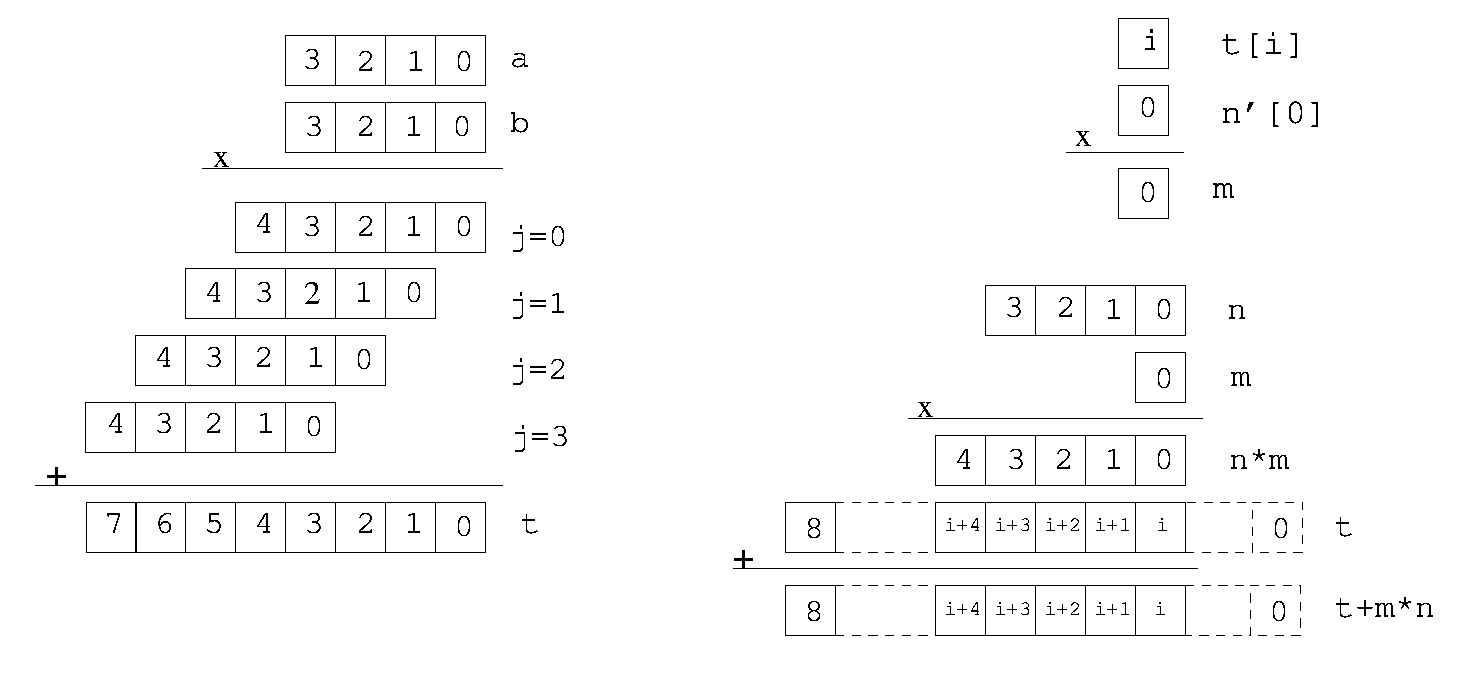
\includegraphics[width=\columnwidth]{sos.eps}
\label{sos}
\end{figure}

The value $n_0'$ is the inverse of the least significant word of $n$
modulo $2^w$, i.e., $n'_0 = -n_0^{-1} \pmod{2^w}$, and can be computed
with a very simple algorithm in \cite{DK90:A}.  By separating $a \cdot
b$ from the rest of the steps for computing $u$, we can optimize the
Montgomery multiplication for squaring when $a=b$. The optimization 
skips almost half of the single-precision multiplications
since $a_i \cdot a_j = a_j \cdot a_i$. The following
simple code replaces the first part of the Mongtomery multiplication
algorithm for optimized Montgomery squaring:
%
\begin{verbatim}
    for i=0 to s-1
        (C,S) := t[i+i] + a[i]*a[i]
        for j=i+1 to s-1
            (C,S) := t[i+j] + 2*a[j]*a[i] + C
            t[i+j] := S
        t[i+s] := C
\end{verbatim}
%
One tricky part here is that the value \texttt{2*a[j]*a[i]} requires
more than two words to store; if the $C$ value does not have an
extra bit, then one way to deal with this is to rewrite the loop
so that the \texttt{a[j]*a[i]} terms are added first, without the multiplication
by $2$; the result is then doubled and the \texttt{a[i]*a[i]} terms are
added in.


\subsubsection{The Coarsely Integrated Operand Scanning (CIOS) Method}
\label{sect-cios}

The Coarsely Integrated Operand Scanning method,
improves on the first one by integrating the multiplication and
reduction steps. Specifically, instead of computing the entire
product $a \cdot b$, then reducing, we alternate between iterations
of the outer loops for multiplication and reduction. We can do this
since the value of $m$ in the $i$th iteration of the outer loop
for reduction depends only on the value \texttt{t[i]}, which is
completely computed by the $i$th iteration of the outer loop for the
multiplication. This leads to the following algorithm:
%
\begin{verbatim}
    t := 0
    for i=0 to s-1
        C := 0
        for j=0 to s-1
            (C,S) := t[j] + a[j]*b[i] + C
            t[j] := S
        (C,S) := t[s] + C
        t[s] := S
        t[s+1] := C
        C := 0
        m := t[0]*n'[0] mod W
        for j=0 to s-1
            (C,S) := t[j] + m*n[j] + C
            t[j] := S
        (C,S) := t[s] + C
        t[s] := S
        t[s+1] := t[s+1] + C
        for j=0 to s
            t[j] := t[j+1]
\end{verbatim}

\noindent
The last $j$-loop is used to shift the result one word to the right
(i.e., division by $2^w$), hence the references to \texttt{t[j]}
and \texttt{t[0]} instead of \texttt{t[i+j]} and \texttt{t[i]}.
A slight improvement is to integrate
the shifting into the reduction as follows:
%
\begin{verbatim}
        m := t[0]*n'[0] mod W
        (C,S) := t[0] + m*n[0]
        for j=1 to s-1
            (C,S) := t[j] + m*n[j] + C
            t[j-1] := S
        (C,S) := t[s] + C
        t[s-1] := S
        t[s] := t[s+1] + C
\end{verbatim}

\noindent
The auxiliary array $t$ uses only $s+2$
words.  This is due to fact that the shifting is done one word
at a time, rather than $s$ words at once, saving $s-1$ words.
The final result is in the first $s+1$ words of array $t$.
A related method, without the shifting of the array (and hence
with a larger memory requirement), is described
as Improvement 2 in \cite{DK90:A}.

The CIOS method (with the slight improvement above)
requires $2s^2+s$ multiplications, $4s^2+4s+2$ additions,
$6s^2+7s+2$ reads, and $2s^2+5s+1$ writes,
including the final multi-precision subtraction, and uses
$s+3$ words of memory space. The memory reduction is a significant
improvement over the SOS method.

We say that the integration in this method is \textit{coarse} because it
alternates between iterations of the outer loop. In the next method,
we will alternate between iterations of the inner loop.


\subsubsection{The Finely Integrated Operand Scanning (FIOS) Method}
\label{sect-fios}

This method integrates the two inner loops of the CIOS method
into one by computing
the multiplications and additions in the same loop.
The multiplications $a_j \cdot b_i$ and $m \cdot n_j$ are
computed in the same loop, and then added to form the final $t$.
In this case, $t_0$ must be computed before entering into the
loop since $m$ depends on this value which corresponds to unrolling
the first iteration of the loop for $j=0$.
%
\begin{verbatim}
    for i=0 to s-1
        (C,S) := t[0] + a[0]*b[i]
        ADD(t[1],C)
        m := S*n'[0] mod W
        (C,S) := S + m*n[0]
\end{verbatim}
%
The partial products of $a\cdot b$ are computed one by one for
each value of $i$, then $m\cdot n$ is added to the partial product.
This sum is then shifted right one word, readying $t$ for the
next $i$-iteration.
%
\begin{verbatim}
        for j=1 to s-1
            (C,S) := t[j] + a[j]*b[i] + C
            ADD(t[j+1],C)
            (C,S) := S + m*n[j]
            t[j-1] := S
        (C,S) := t[s] + C
        t[s-1] := S
        t[s] := t[s+1] + C
        t[s+1] := 0
\end{verbatim}

The FIOS method has only one inner loop when compared to CIOS.  We
illustrate the algorithm in Figure~\ref{fios} for $s=4$.  The
use of the {\tt ADD} function is required in the inner $j$-loop since
there are two distinct carries, one arising from the multiplication of
$a_j\cdot b_i$ and the other from the multiplication of $m\cdot n_j$.
(Thus the benefit of having only one loop is counterbalanced by the
requirement of the {\tt ADD} function.) The array $t$ is assumed to be
set to 0 initially.

\begin{figure}[ht]
\caption[An iteration of the Finely Integrated Operand Scanning (FIOS) method.]
{An iteration of the Finely Integrated Operand Scanning (FIOS) method.
The computation of partial product $\,t^{(i)}=a\times b_i\,$,
illustrated on the left, enables the computation of $\,m^{(i)}$ in
that iteration. Then an intermediate result $\,t^{(i+1)}\,$ is
found by adding $n\times m^{(i)}$ to this partial product,
as shown on the right.}
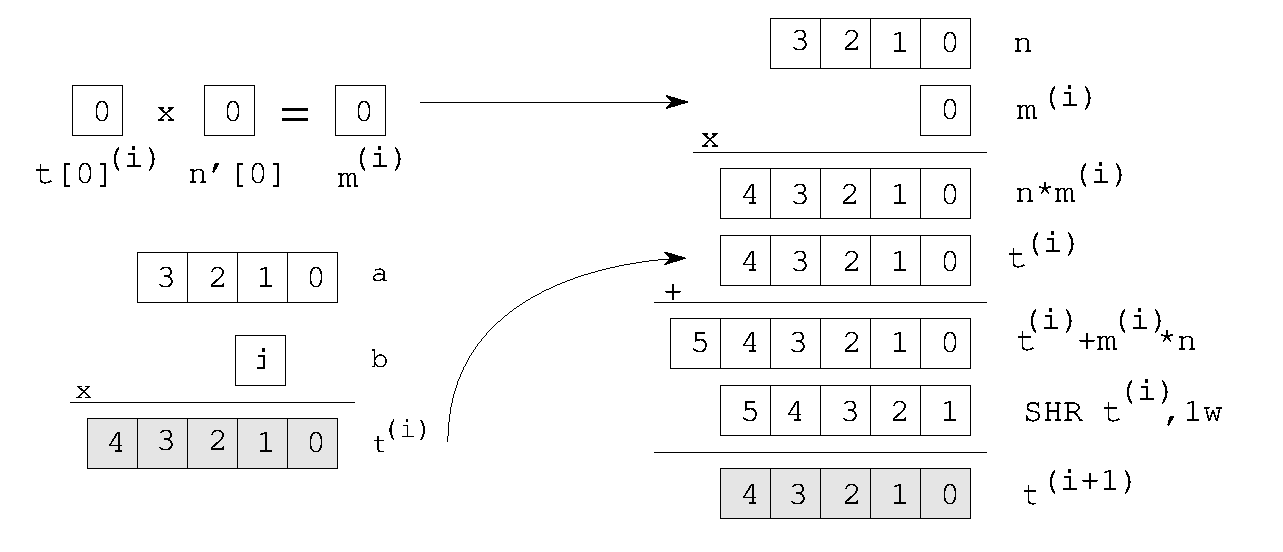
\includegraphics[width=\columnwidth]{fios.eps}
\label{fios}
%\epsfxsize=4.3in    % 21.5 squares, 1 square=0.2in
%\centerline{\epsfbox{chapter2/fios.eps}}
\end{figure}

The FIOS
method requires $2s^2+s$ multiplications,
$5s^2+3s+2$ additions, $7s^2+5s+2$ reads,
and $3s^2+4s+1$ writes, including the final multi-precision subtraction.
This is about $s^2$ more additions, writes, and reads than for
the CIOS method.
The total amount of temporary space required is $s+3$ words.


\subsubsection{The Finely Integrated Product Scanning (FIPS) Method}
\label{sect-fips}

Like the previous one, this method interleaves the computations
$a\cdot b$ and $m \cdot n$, but here both computations are in the
product-scanning form. The method keeps the values of $m$ and $u$ in
the same $s$-word array $m$.  This method was described in
\cite{K93:The} and is related to Improvement 3 in \cite{DK90:A}.  The
first loop given below computes one part of the product $a\cdot b$ and
then adds $m\cdot n$ to it.  The three-word array $t$, i.e.,
%
\begin{verbatim}
    t[0], t[1], t[2],
\end{verbatim}
%
is the partial product accumulator for  $a\cdot b$
and $m\cdot n$. The use of a three-word array assumes 
$s < W$; in general, we need $\log_W (sW(W-1)) \approx 2 + \log_W s$
words. The algorithm is easily modified to handle a larger
accumulator.
%
\begin{verbatim}
    for i=0 to s-1
        for j=0 to i-1
            (C,S) := t[0] + a[j]*b[i-j]
            ADD(t[1],C)
            (C,S) := S + m[j]*n[i-j]
            t[0] := S
            ADD(t[1],C)
        (C,S) := t[0] + a[i]*b[0]
        ADD(t[1],C)
        m[i] := S*n'[0] mod W
        (C,S) := S + m[i]*n[0]
        ADD(t[1],C)
        t[0] := t[1]
        t[1] := t[2]
        t[2] := 0
\end{verbatim}
%
In this loop, the $i$th word of $m$ is computed using $n_0'$, and the
least significant word of $m \cdot n$ is added to $t$. Since the least
significant word of $t$ always becomes zero, eash iteration shifts one
word at a time.  The array $t$ is set to 0 initially.

The second $i$-loop, given below, completes the final result $u$ word
by word in the memory space of $m$.
%
\begin{verbatim}
    for i=s to 2s-1
        for j=i-s+1 to s-1
            (C,S) := t[0] + a[j]*b[i-j]
            ADD(t[1],C)
            (C,S) := S + m[j]*n[i-j]
            t[0] := S
            ADD(t[1],C)
        m[i-s] := t[0]
	m[i-s+1] := t[1]
        t[0] := t[1]
        t[1] := t[2]
        t[2] := 0
\end{verbatim}
%
An inspection of indices in the second $i$-loop reveals that the least
significant $s$ words of the result $u$ are located in $m$. The most
significant bit is in \texttt{t[0]}. The values \texttt{t[1]} and
\texttt{t[2]} are zero at the end: a good place for \texttt{assert()}.

The FIPS method requires $2s^2+s$ multiplications, $6s^2+2s+2$
additions, $9s^2+8s+2$ reads, and $5s^2+8s+1$ writes. The number of
additions, reads and writes is somewhat more than the previous
methods, but the number of multiplications is the same.  The method
may have considerable benefits on digital signal processors.
%, as discussed in Section \ref{conclusion}. 
Note that many of the
reads and writes are for the accumulator words, which may be in
registers.  The space required is $s+3$ words.


\subsubsection{The Coarsely Integrated Hybrid Scanning (CIHS) Method}
\label{sect-cihs}

This method is a modification of the SOS method, illustrating yet
another approach to Montgomery multiplication.  Here we show that it
is possible to use only $s+3$ words of temporary memory without
changing the general flow of the algorithm.  We call it a \textit{hybrid
  scanning} method because it mixes the product-scanning and
operand-scanning forms of multiplication.  Reduction is just in the
operand-scanning form.  First, we split the computation of $a \cdot
b$ into two loops.  The second loop shifts the intermediate result one
word at a time at the end of each iteration.

The splitting of multiplication is possible because $m$ is computed by
multiplying the $i$th word of $t$ by $n_0'$.  Thus, the multiplication
$a\cdot b$ can be simplified by postponing the word multiplications
required for the most significant half of $t$ to the second $i$-loop.
The multiplication loop can be integrated into the second main
$i$-loop, computing one partial product in each iteration and reducing
the space for the $t$ array to $s+2$ words from $2s+1$ words.  In the
first stage, $(n-j)$ words of the $j$th partial product of $a\cdot b$
are computed and added to $t$. In Figure~\ref{cihs}, the
computed parts of the partial products are shown by straight lines,
and the added result is shown by shaded blocks. This computation can
be performed using the following code:
%
\begin{verbatim}
    for i=0 to s-1
        C := 0
        for j=0 to s-i-1
            (C,S) := t[i+j] + a[j]*b[i] + C
            t[i+j] := S
        (C,S) := t[s] + C
        t[s] := S
        t[s+1] := C
\end{verbatim}

\begin{figure}[ht]
\caption[An iteration of the Coarsely Integrated Hybrid Scanning (CIHS)
method.]
{An iteration of the the Coarsely Integrated Hybrid Scanning (CIHS)
method for $s=4$.
%
The left-hand side figure shows the
accumulation of the right half of the partial products $a\times b$
which is in the first $i$-loop.
%
The second $i$-loop is depicted in two parts in the middle and the
right.  The addition of $n\times m$ to $t$ and the shifting of
$t+m\times n$ are illustrated in the middle, which are
in the first $j$-loop of the second $i$-loop.
%
The computation of the remaining words of the partial products of
$a\times b$ is illustrated on the right-hand side.  Each (PC,PS) pair
is the sum of the columns connected with lines.
%
As illustrated in the bottom of the middle part, the (PC,PS) pair is
added to $t^{(i)}$, which is performed in the last $j$-loop.}
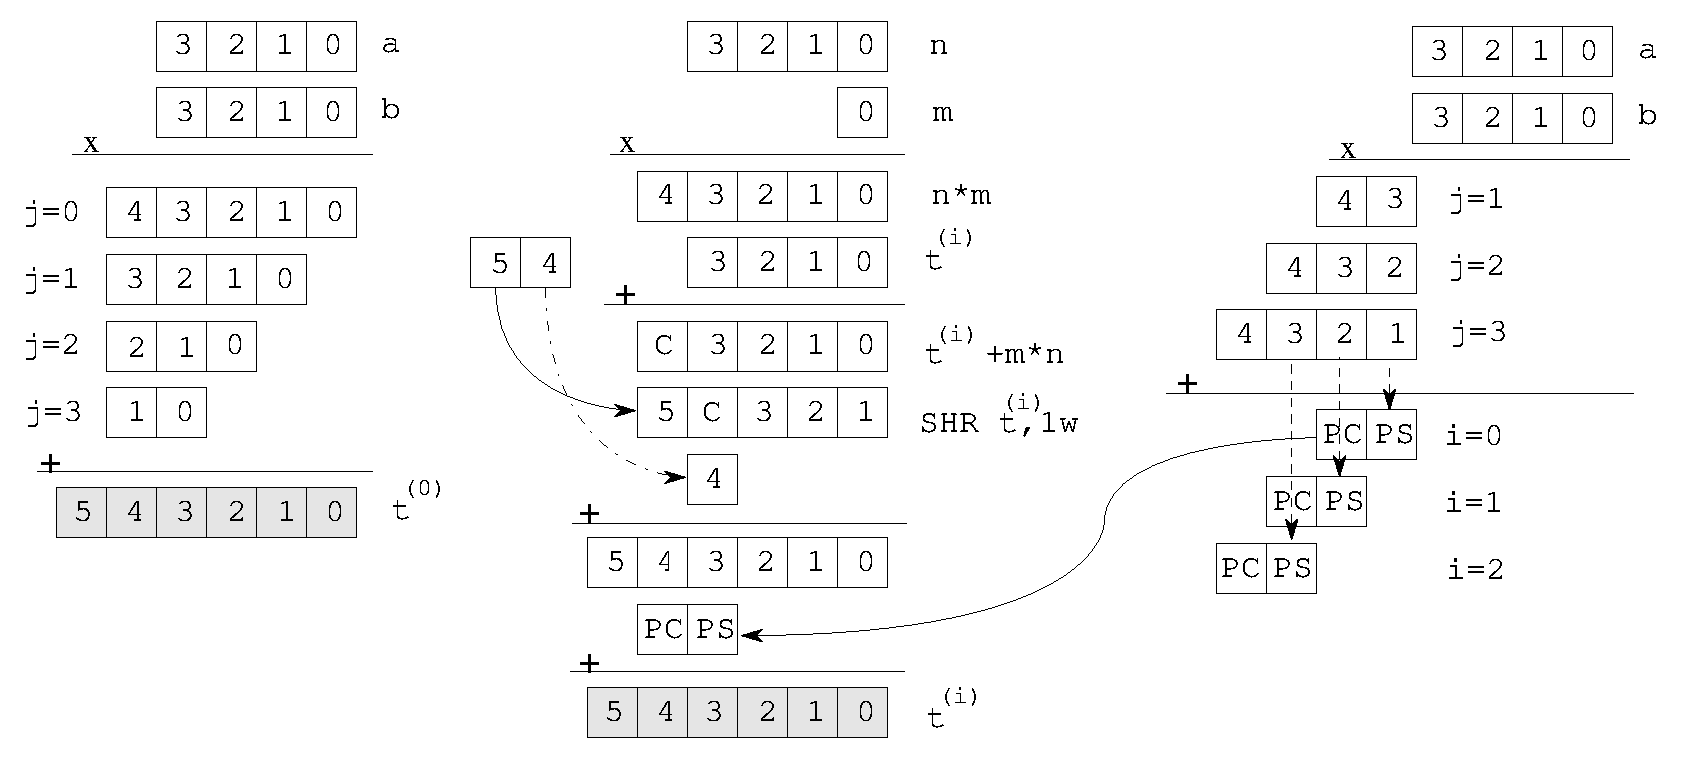
\includegraphics[width=\columnwidth]{cihs.eps}
\label{cihs}
%\epsfxsize=5.6in      % 28 squares, 1 square 0.2
%\centerline{\epsfbox{chapter2/cihs.eps}}
\end{figure}

\noindent
The multiplication of $m\cdot n$ is then interleaved with
the addition $a \cdot b + m \cdot n$. The division by $r$ is performed
by shifting one word at a time within the $i$-loop.
Since $m$ is one word long and the product $m\cdot n+C$ is two words long,
the total sum $t + m\cdot n$ needs at most $s+2$ words.
Also note that the carry propagation into the $s$th word is performed into
the $(s-1)$st word after the shifting. The array $t$ is assumed
to be set to 0 initially.
%
\begin{verbatim}
    for i=0 to s-1
        m := t[0]*n'[0] mod W
        (C,S) := t[0] + m*n[0]
        for j=1 to s-1
            (C,S) := t[j] + m*n[j] + C
            t[j-1] := S
        (C,S) := t[s] + C
        t[s-1] := S
        (C,S) := t[s+1] + C
        t[s] := S
        t[s+1] := C
\end{verbatim}
%
The computation of $m$ requires the use of $t_0$ instead
of $t_i$, as in the original SOS algorithm.
This is due to the shifting of $t$ in each iteration.
The two excess words computed in the first loop are used in the
following $j$-loop which computes the $(s+i)$th word of
$a\cdot b$.
%
\begin{verbatim}
        for j=i+1 to s-1
            (C,S) := t[s-1] + b[j]*a[s-j+i]
            t[s-1] := S
            (C,S) := t[s] + C
            t[s] := S
            t[s+1] := t[s+1] + C
\end{verbatim}
%
We note that the above four lines compute the most significant three words of
$t$, i.e., the $(s-1)$st, $s$th, and $(s+1)$st words of $t$. The
above code completes Step 1 of $\mon(a,b)$. After this, $n$ is
subtracted from $t$ if $t\geq n$. We illustrate the algorithm in
Figure~3 for Montgomery multiplication of two four-word numbers.

Symbols PC and PS denote the two extra words
required to obtain the correct $(s+i)$th word.
Each PC, PS pair is the sum of their respective words connected by
vertical dashed lines in Figure~3.
The number of multiplications required in this method is also equal to
$2s^2+s$. However, the number of additions decreases to $4s^2+4s+2$.
The number of reads is $6.5s^2+6.5s+2$ and the number of
writes is $3s^2+5s+1$.
This algorithm requires $s+3$ words of temporary memory.

\subsection{Vectorized Implementations}
\label{vectorized}

Montgomery multiplication can also be implemented with SIMD instructions
such as Intel and ARM SSE instructions \cite{GK12:Software,BMZS13:Montgomery}.
The SIMD implementation exploits the micro-parallelism to provide a 1.5 speed-up.

Starting with the following unmodified algorithm,
Montgomery, et.al. parallelized the Montgomery algorithm with two way SIMD instructions.
%
\begin{tabbing}
\hspace*{0.2in} \= \hspace*{0.5in}\=\\
\> 1. $t := 0$ \\
\> 2. \bfor $i=0$ to $n-1$ do \\
\> 3. \> $t := t + a_i\cdot B$ \\
\> 4. \> $m := n_0' \cdot t \bmod r$ \\
\> 5. \> $t := (t + m\cdot n)/r$ \\
\> 6. \bif $t \geq M$ \bthen \\
\> 7. \> $t := t - M$ \\
\> 8. return $t$
\end{tabbing}

In this algorithm, observe that lines 3, 4, and 5 can be replaced with the following two lines
to ensure that the two larger multiplications don't depend on each other.
A minor change is to use $n_0^{-1} \bmod r$ instead of $-n_0^{-1} \bmod r$ for $n_0'$.
\begin{eqnarray*}
m & := &  ((t_0 + a_i\cdot b_0)\cdot n_0') \bmod r \\
t  & := & (t + a_i\cdot B + m\cdot n) / r
\end{eqnarray*}

The final algorithm steps are described in two computations of $D$ and $E$ values that are
combined at the end to get $t$. The conditional subtraction is also replaced by a conditional addition if $t<0$.
The final algorithm is Algorithm 2 in \cite{BMZS13:Montgomery}.
The instruction counts also change and are given in the same publication on Table~\ref{simdCounts}.

\begin{table}
\caption{SIMD implementation instruction counts.}
\label{simdCounts}
\begin{tabular}{|l||c|c|c|} \hline
Instr. & 32-bit & 64-bit & SIMD2-32 \\
\hline\hline
\texttt{add} & - & - & $n$ \\
\texttt{sub} & - & - & $n$ \\
\texttt{shortmul} & $n$ & $n/2$ & $2n$ \\
\texttt{muladd} & $2n$ & $n$ & - \\
\texttt{muladdadd} & $2n(n-1)$ & $n(n/2-1)$ & - \\
\texttt{SIMD-muladd} & - & - & $n$ \\
\texttt{SIMD-muladdadd} & - & - & $n(n-1)$ \\
\hline
\end{tabular}
\end{table}
%
\noindent
The 32-bit and 64-bit counts reflect an ALU-only implementation as described previously where the word size is 32 bits.
SIMD2-32 means two-way SIMD with 32-bit words a supported by Intel and ARM CPUs.

\section{Software Implementations}
\label{sec:softimp}

In this section, we will present detailed information about implementation of Modular Multiplication on software. To achieve efficient implementations, we utilize the integer instruction extensions of Intel architecture added to the new generation processor cores~\cite{largeint}. Implementation was done in Intel x64 assembly code because multiplication operations require efficient carry chain implementations only possible via assembly coding.

Figure \ref{fig:mult} shows only a breakdown of multiplication of large numbers. The $A_iB$ multiplication needs a closer examination in order to describe the multiplication of a large number by one word.
%
The algorithm starts off with the first diagonal to compute the first partial product.
The remaining diagonals add the intermediate products to the previous diagonal's result, essentially accumulating
partial products into the final result.
%
Figure \ref{fig:diag0} depicts the detailed multiplication steps of the first diagonal in a 512x64 bit multiplication.

\begin{figure}[ht]
\centering
  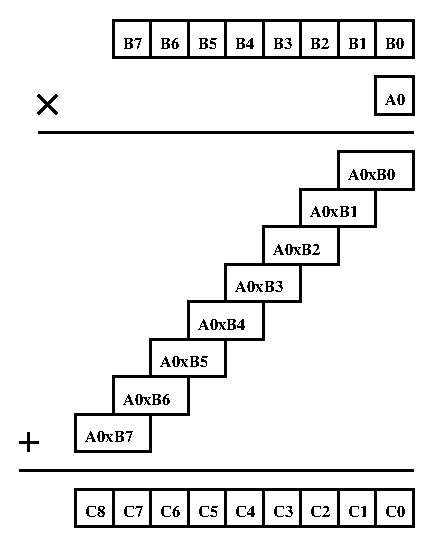
\includegraphics[scale=0.7]{multdiag0.eps}
\caption{First diagonal of a 512x64 bit multiplication operation}
\label{fig:diag0}
\end{figure}

What follows below, each multiplication is a 64x64 core multiplication and each result is a 128-bit integer.
%
Low 64 bits of each result is stored in \texttt{rax} and high 64 bits of each result is stored in \texttt{rdx}. A code snippet for the first diagonal is given below.


\begin{verbatim}
mov rbp, [A + 8*0]
mov rax, [B + 8*0]
mul rbp

mov [C + 8*0], rax
mov R0, rdx

mov rax, [B + 8*1]
mul rbp
add R0, rax
adc rdx, 0
mov R1, rdx
...
...
mov rax, [B + 8*6]
mul rbp
add R5, rax
adc rdx, 0
mov R6, rdx

mov rax, [B + 8*7]
mul rbp
add R6, rax
adc rdx, 0
mov R7, rdx
\end{verbatim}

Here, it can be seen that the result \texttt{C0} is stored in memory, since it doesn't change after this diagonal is completed. Results \texttt{C1} through \texttt{C8} are stored in registers \texttt{R0} through \texttt{R7} to avoid load-store operations. One of the operands of the \texttt{mul} instruction is implicitly stored in register \texttt{rax} and the other operand is stored in any register. The product is stored in registers \texttt{rdx} and \texttt{rax}. 
\begin{verbatim}
mul src
{rdx,rax} = src*rax
\end{verbatim}
defines the multiply operation. This instruction has two main flaws: Requires the outputs moved to other registers once the multiplication is completed, as the next multiplication would destroy the current result and the mul instruction destroys all of the flags.
%
The new Intel instruction \texttt{mulx} provides relief as follows:
\begin{verbatim}
mulx dest_hi, dest_lo, src1
dest_hi:dest_lo = src1 * rdx.
\end{verbatim}
The new \texttt{mulx} instruction was introduced in the 4th generation Intel cores (formerly known as Haswell). In addition to explicit destination registers, it does not destroy the carry flag, and allows a better code sequence as shown below for the first diagonal multiplication.
\begin{verbatim}
mov rdx , [A + 8*0]
mulx R0 , rax , [B + 8*0]
mov [C + 8*0] , rax
mulx R1 , rax , [B + 8*1]
add R0 , rax
mulx R2 , rax , [B + 8*2]
adc R1 , rax
...
...
mulx R6 , rax , [B + 8*6]
adc R5 , rax
mulx R7 , rax , [B + 8*7]
adc R6 , rax
adc R7 , 0
\end{verbatim}

After the first diagonal, we have an intermediate result where subsequent partial products in diagonal multiplications are accumulated into. Figure \ref{fig:diag1} gives the second diagonal's multiplication details of a 512x64 bit multiplication. The rest of the diagonals behave exactly the same way.

\begin{figure}[ht]
\centering
  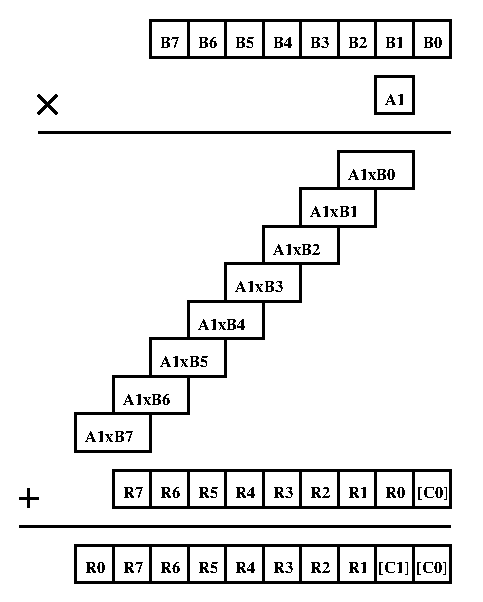
\includegraphics[scale=0.7]{multdiag1.eps}
\caption{Second diagonal of a 512x64 bit multiplication operation}
\label{fig:diag1}
\end{figure}

Next, we show how to add three numbers the \texttt{mul} output: 
high part of the previous result, low part of the current result, and corresponding intermediate result.

\begin{verbatim}
mov rbp, [A + 8*0]
mov rax, [B + 8*0]
mul rbp	
add	R0, rax
adc rdx, 0
mov [C + 8*0], R0
mov rbx, rdx

mov rax, [B + 8*1]
mul rbp
mov R0, rdx
add R1, rax
adc R0, 0
add R1, rbx
adc R0, 0
...
...
mov rax, [B + 8*7]
mul rbp
mov R0, rdx
add R7, rax
adc R0, 0
add R7, rbx
adc R0, 0
\end{verbatim}

Figure \ref{fig:diag1} shows two seperate carry chains.
Not surprisingly, Intel provided relief with two more new instructions: \texttt{adcx} and \texttt{adox} as follows.

\begin{verbatim}
adcx dest/src1, src2
adox dest/src1, src2
\end{verbatim}

The \texttt{adcx} instruction operates exactly same way as the \texttt{adc} instruction, except that it does not alter the overflow flag (OF).
The \texttt{adox} instruction operates exactly same way as the \texttt{adc} instruction, but uses the OF as its carry flag and does not change the carry flag (CF). This allows parallel execution of two seperate carry chains. This is realized with code sequence below. 

\begin{verbatim}
xor rax , rax
mov rdx , [A + 8*0]
mulx rbx , rbp , [B + 8*0]
adox R0 , rbp
adcx R1 , rbx
mov [C + 8*0] , R0
mulx rbx , R0 , [B + 8*1]
adox R0 , R1
adcx R2 , rbx
...
...
mulx rbx , R5 , [B + 8*6]
adox R5 , R6
adcx R7 , rbx
mulx rbx , R6 , [B + 8*7]
adox R6 , R7
adcx rbx , rax
adox rbx , rax
mov R7 , rbx
\end{verbatim}

This section provides details of large number multiplications with the new instructions.
The reduction can be implemented very efficiently similar to multiplication using the same techniques
which we omit for brevity.

\section{Implementation Results}
\label{sec:res}

\begin{table*}[ht]
\caption{Implementation Results}
\label{table:impres}
\begin{center}
\begin{tabular}{|c|c|c|c|c|c|}
\hline
\multicolumn{2}{|c|}{}	& \multicolumn{2}{c|}{$4^{th}$ Generation CPU} & \multicolumn{2}{c|}{$6^{th}$ Generation CPU} \\
\multicolumn{2}{|c|}{}	& \multicolumn{2}{c|}{i7-4770} & \multicolumn{2}{c|}{i7-6700HQ} \\
\cline{3-6}
\multicolumn{2}{|c|}{}	& Latency & Cycle/mul & Latency & Cycle/mul \\
\hline
 & pre-HSW ISA & 134 & 2.09 & 133 & 2.08 \\
\cline{2-6}
512x512 Multiplication & with mulx & 126 & 1.96 & 123 & 1.92 \\
\cline{2-6}
 & with adcx/adox &  &  & 95 & 1.48 \\
\hline
 & pre-HSW ISA & 317 & 2.33 & 276 & 2.03 \\
\cline{2-6}
512x512 Modular Multiplication & with mulx & 270 & 1.99 & 266 & 1.96 \\
\cline{2-6}
 & with adcx/adox &  &  & 195 & 1.43 \\
\hline
\end{tabular}
\end{center}
\end{table*}

We implemented Montgomery Multiplication and Montgomery Reduction using x64 Intel Assembly Language. We employed the aforementioned instruction extensions to accelerate public-key cryptography operations.
We ran our experiments on a 4th generation i7-4770 CPU clocked at 3.4 GHz, and 6th generation i7-6700HQ CPU running clocked at 2.6 GHz for benchmarking.
%
Benchmarking tends to have numerous tricks and tweaks. To reduce the number of variable knobs,
we disabled Turbo Boost. Results are shown in Table \ref{table:impres}. We have three different implementations for Montgomery Multiplication of two 512-bit numbers. The first implementation does not utilize any instruction extensions, which we call pre-HSW ISA (Instruction Set Architecture). The second and third implementations use \texttt{mulx} and \texttt{adcx/adox} instructions, respectively.


\section{Conclusion}
\label{sec:conc}
There are several ways to implement the Montgomery reduction algorithm
which started with Peter's short but landmark paper.
We analyzed several of these algorithms for run-time efficiency
and provided benchmark results for Intel and ARM architectures.
We caution the reader to dig deeper: there is more than converting algorithm
descriptions and code snippets to secure cryptographic algorithm implementations,
e.g., potentially devastating side-channel leakage.
With that in mind, we close with an observation and relay our experience to conclude
that Montgomery multiplication is still very effective after three decades,
and continues to be the algortihm of choice for many cryptographic algorithms on modern platforms.

%\subsection{Results and Conclusions}
%\label{conclusion}
%
%The algorithms presented in this chapter require the same number of
%single-precision multiplications, but the number of additions,
%reads and writes are slightly different.  There seems to be a lower
%bound of $4s^2+4s+2$ for additions that the SOS and CIOS
%methods reach.  The number of operations and the
%amount of temporary memory  are summarized in
%Table~\ref{requirements}. The total number of operations is
%calculated by counting each operation within a loop, and multiplying
%this number by the iteration count. As an example we illustrate the
%calculation for the CIOS method in Table~\ref{cios-operations}.
%
%\begin{table*}
%\caption{The time and space requirements of the methods.}
%\label{requirements}
%\begin{tabular}{|l||c|l|l|l||r|} \hline
%Method & Multiplications & Additions & Reads & Writes & Space \\
%\hline\hline
%SOS    & $2s^2+s$ & $4s^2+4s+2$ & $6s^2+7s+3$ & $2s^2+6s+2$ & $2s+2$ \\
%CIOS   & $2s^2+s$ & $4s^2+4s+2$ & $6s^2+7s+2$ & $2s^2+5s+1$ & $s+3$ \\
%FIOS   & $2s^2+s$ & $5s^2+3s+2$ & $7s^2+5s+2$ & $3s^2+4s+1$ & $s+3$ \\
%FIPS   & $2s^2+s$ & $6s^2+2s+2$ & $9s^2+8s+2$ & $5s^2+8s+1$ & $s+3$ \\
%CIHS   & $2s^2+s$ & $4s^2+4s+2$ & $6.5s^2+6.5s+2$ & $3s^2+5s+1$ & $s+3$ \\
%\hline
%\end{tabular}
%\end{table*}
%
%We note that the \texttt{ADD(x[i],C)} function, which implements the
%operation \texttt{x[i] := x[i] + C} including the carry propagation,
%requires one memory read (\texttt{x[i]}), one addition
%(\texttt{x[i]+C}) and one memory write (\texttt{x[i]:=}) operation
%during the first step.  Considering the carry propagation from this
%addition, on average one additional memory read, one addition, and one
%memory write will be done in addition to the branching and loop
%instructions.  Thus, the \texttt{ADD} function requires two
%memory reads, two additions, and two memory writes in our analysis.
%
%\begin{table*}
%\caption{Calculating the operations of the CIOS method.}
%\label{cios-operations}
%\small
%\begin{tabular}{|l|c|c|c|c|c|}
%\hline
%& \multicolumn{4}{c|}{\small Operation} & \\
%\cline{2-5}
%{\small\bf STATEMENT} &
%\small Mult & \small Add & \small Read & \small Write &
%  \small Iterations \\ \hline
%\scriptsize\verb%for i=0 to s-1% &
%- & - & - & - & -  \\
%\scriptsize\verb%  C := 0% &
%0 & 0 & 0 & 0 & $ s$\\
%\scriptsize\verb%  for j=0 to s-1% &
%- & - & - & - & - \\
%\scriptsize\verb%    (C,S) := t[j] + b[j]*a[i] + C% &
%1 & 2 & 3 & 0 & $s^2$ \\
%\scriptsize\verb%    t[j] := S% &
%0 & 0 & 0 & 1 & $s^2$ \\
%\scriptsize\verb%  (C,S) := t[s] + C% &
%0 & 1 & 1 & 0 & $s$ \\
%\scriptsize\verb%  t[s] := S% &
%0 & 0 & 0 & 1 & $s$ \\
%\scriptsize\verb%  t[s+1] := C% &
%0 & 0 & 0 & 1 & $s$ \\
%\scriptsize\verb%  m := t[0]*n'[0] mod W% &
%1 & 0 & 2 & 1 & $s$ \\
%\scriptsize\verb%  (C,S) := t[0] + m*n[0]% &
%1 & 1 & 3 & 0 & $s$ \\
%\scriptsize\verb%  for j=1 to s-1% &
%- & - & - & - & - \\
%\scriptsize\verb%    (C,S) := t[j] + m*n[j] + C% &
%1 & 2 & 3 & 0 & $s(s-1)$  \\
%\scriptsize\verb%    t[j-1] := S% &
%0 & 0 & 0 & 1 & $s(s-1)$ \\
%\scriptsize\verb%  (C,S) := t[s] + C% &
%0 & 1 & 1 & 0 & $s$ \\
%\scriptsize\verb%  t[s-1] := S% &
%0 & 0 & 0 & 1 & $s$ \\
%\scriptsize\verb%  t[s] := t[s+1] + C% &
%0 & 1 & 1 & 1 & $s$  \\
%\small Final Subtraction &
%0 & $ 2(s+1)$ & $ 2(s+1)$ & $ s+1$ & 1  \\
%\cline{2-6}
%& $2s^2+s$ & $4s^2+4s+2$ & $6s^2+7s+2$ & $2s^2+5s+1$ & \\ \hline
%\end{tabular}
%\end{table*}
%
%Our counting is a first-order approximation; we are not
%taking into account the full use of registers to store intermediate
%values, cache size in the data and instruction misses, and the special
%instructions such as multiply and accumulate.
%We have also not counted loop overhead, pointer arithmetic, and the
%like, which would undoubtedly affect performance.
%Implementation results are published in \cite{KAK96:Analyzing}.
%
%
%In the C version of the functions, single-precision multiplications
%are done by dividing them into two half words.  The C version has more
%overhead compared to the assembler version, in which one-word
%multiplicationd are carried out using a single assembler instruction.
%The assembler version of the {\tt ADD} function is optimized to use
%one register for addition and another register for address
%computation.  The propagation of the carry is performed using the
%carry flag.
%
%The CIOS and FIOS methods are similar to
%one another in their use of embedded shifting and interleaving the
%products $a_i\cdot b$ and $m\cdot n_j$. The only difference is that
%CIOS method computes the partial product $a_i\cdot b$ by
%using a separate $j$-loop. Then, the accumulation of $m\cdot n_j$ to
%this partial product is performed in the succeeding $j$-loop.
%The FIOS method combines the computation of partial
%product $a_i\cdot b$ and accumulation of $a_i\cdot b$ and $m\cdot n_j$
%in one single $j$-loop, thereby obligating the use of the {\tt ADD}
%function for propagation of two separate carries.
%
%The CIOS algorithm operated faster on Intel processors with non-SSE
%instructions compared to the other Montgomery multiplication
%algorithms, especially when implemented in assembly language. However,
%on other classes of processors, a different algorithm may be
%preferable.  For instance, on a digital signal processor, we have
%often found the FIPS method to be better because it exploits the
%\textit{multiply-accumulate} architecture typical with such processors,
%where a set of products are added together. On such architectures, the
%three words $t[0]$, $t[1]$ and $t[2]$ are stored in a single hardware
%accumulator, and the product \texttt{a[j]*b[i-j]} in the FIPS $j$-loop
%can be added directly to the accumulator, which makes the $j$-loop
%very fast.
%
%On a general-purpose processor, the CIOS and the FIOS algorithms seem
%like the best choices. They are simple and require relatively fewer
%additions and fewer assignments. 


\begin{acknowledgements}
The authors express their thanks to Dan Shumow and Greg Zaverucha for their vectorized
algorithm descriptions.
\end{acknowledgements}


% BibTeX users please use one of
%\bibliographystyle{spbasic}      % basic style, author-year citations
\bibliographystyle{spmpsci}      % mathematics and physical sciences
%\bibliographystyle{spphys}       % APS-like style for physics
\bibliography{tolga}   % name your BibTeX data base

\end{document}
